\documentclass[a4paper,11pt]{article}
\usepackage{a4wide,ngerman,url,graphicx}
\usepackage[utf8]{inputenc}
\parskip4pt
\parindent0pt

\title{Analyse der Coronastatistiken} 
\author{Hans-Gert Gräbe, Leipzig}
\date{Version vom 30. März 2020}

\begin{document}
\maketitle

Dieser Text beschreibt die im Verzeichnis
\begin{center}
  \url{http://leipzig-netz.de/MINT/Corona-20/}
\end{center}
verfügbaren Materialien. 

\section{Datenbasis}

Als neue Datenbasis werden die von der John Hopkins Universität im
github-Projekt \url{https://github.com/CSSEGISandData/COVID-19} als
Excel-Datei veröffentlichten Daten zur Entwicklung der weltweit registrierten
Covid-19-Fälle (Stand 28.03.2020) verwendet. Die Statistik listet pro Land und
Tag die kumulative Zahl der Infizierten, die Zahl der Genesenen und die Zahl
der Todesfälle auf.  Aus diesen Tabellen werden mit \texttt{make} Tabellen für
Deutschland, Italien, Spanien und Österreich extrahiert, diese mit dem
php-Skript \texttt{csv2rdf.php} für die weitere Analyse aufbereitet und in der
Datei \texttt{BasicData.txt} gespeichert.

\section{Datentransformation}

Die weitere Verarbeitung wird mit dem freien CAS \emph{Maxima}\footnote{Siehe
  dazu \url{http://maxima.sourceforge.net/de/}, das CAS ist in
  Linux-Distributionen über den Paketmanager leicht zu installieren.}
ausgeführt, wofür in der Datei \texttt{BasicData.txt} die Daten bereits als
Listen von Paaren $(t,c_t)$ gespeichert sind, wobei $t$ den Tag des Jahres
($0=01.01.2020$) und $c_t$ die Zahl der registrierten Neuinfektionen an diesem
Tag angibt. Die Verarbeitung erfolgt mit dem Maxima-Skript \texttt{skript.m}.
Dies ist eine reine Textdatei.

Da mich die kumulative Entwicklung interessiert, sind zunächst diese Daten in
kumulative Daten umzurechnen und als Liste von Paaren $(t,s_t)$ zu speichern.

\section{Fitting}

Alle Grafiken zu Prognosen der kumulativen Daten, die ich bisher gesehen habe,
gehen von einer „Glockenkurve“ aus.  Das ist natürlich in dem hier
entwickelten Datenmodell vollkommen unmöglich, da nach Konstruktion $s_t$ eine
monoton wachsende Folge ist. Wenn die Zahlen wieder zurückgehen, dann müsste
die Zahl der Fälle, die aus der Statistik herausfallen, abgezogen werden.  Ich
gehe aber davon aus, dass diese Zahlen in der Phase des Anrollens der Pandemie
vernachlässigt werden können.

Zur Abschätzung des Verlaufs längs einer Glockenkurve wird üblicherweise die
Statistikfunktion $f(t)=C\exp\left(-\frac{(t-m)^2}{\sigma}\right)$ verwendet,
die ich als Kurvenschar $f(t)=\exp\left(c-s(t-m)^2\right)$ ansetze.

Nun sind die Parameter $(c,s,m)$ dieser Kurvenschar so zu fitten, dass die
ermittelte Kurve besonders gut auf die Daten passt.  In \emph{Maxima} kann
dazu das Paket \emph{lsquares} verwendet werden.

Fitting auf komplizierte Kurvenscharen ist eine schwierige und numerisch wenig
stabile Aufgabe, so auch in diesem Fall. \emph{Maxima} kommt beim Fittung der
Schar $f(t)$ zu keinem Ergebnis.  Einen einfacheren, nämlich quadratischen
Zusammenhang $g(t)=c-s\dot(t-m)^2$ erhält man, wenn man zu Paaren
$(t,\log(s_t))$ übergeht.  Damit lassen sich dann die Fittingparameter stabil
berechnen.

Ein zweites Problem ist die Frage, welche Datenpunkte für ein gutes Fitting
aussortiert werden sollten.  Hier stellte sich heraus, dass beste
Übereinstimmung der Daten mit der Schätzung erzielt wird, wenn nur Daten mit
$s_t>10^3$ (nach Einbezug von Österreich geändert) berücksichtigt werden.

Details sind im Skript \texttt{skript.m} zu finden.

\section{Ergebnisse}

Damit lassen sich Szenarien (!) für die Länder Deutschland, Italien, Spanien
und Österreich erstellen, siehe die Abbildungen.

\begin{figure}
  \begin{center}
    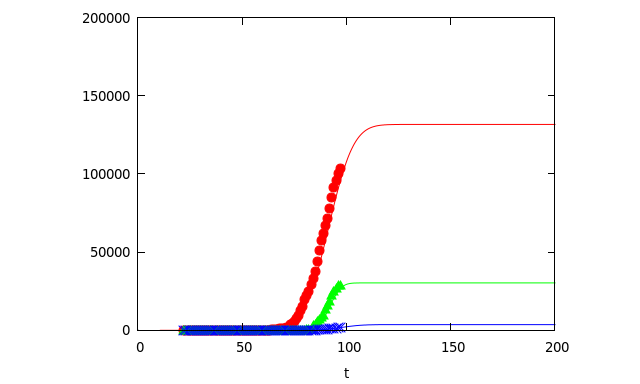
\includegraphics[width=.8\textwidth]{Germany.png}
    \caption{Szenario für Deutschland (82.9 Mio. Einwohner)}
  \end{center}
\end{figure}
\begin{figure}
  \begin{center}
  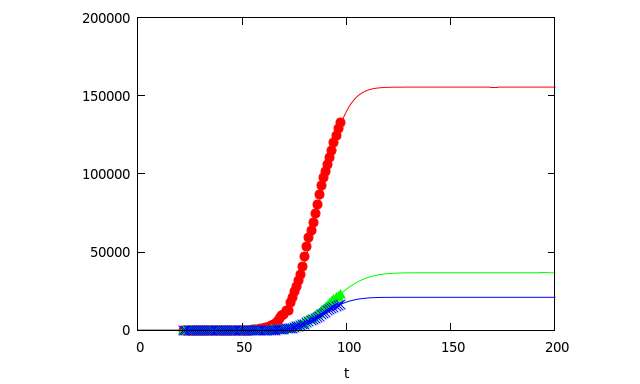
\includegraphics[width=.8\textwidth]{Italy.png}
    \caption{Szenario für Italien (60.4 Mio. Einwohner)}
  \end{center}
\end{figure}
\begin{figure}
  \begin{center}
  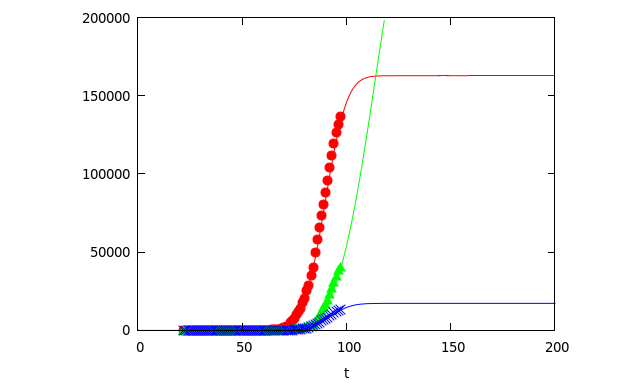
\includegraphics[width=.8\textwidth]{Spain.png}
    \caption{Szenario für Spanien (46.7 Mio. Einwohner)}
\end{center}
\end{figure}

\begin{figure}
  \begin{center}
  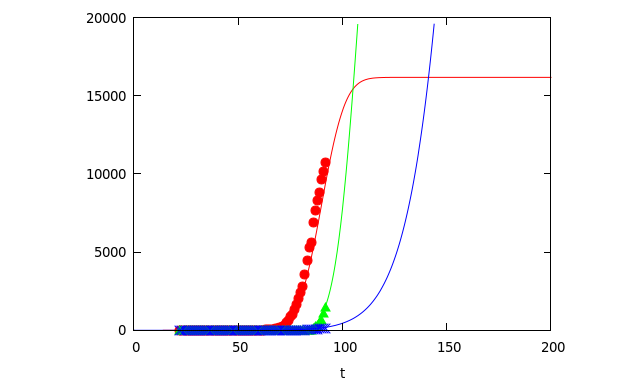
\includegraphics[width=.8\textwidth]{Austria.png}
    \caption{Szenario für Österreich (8.85 Mio. Einwohner)}
\end{center}
\end{figure}

Die berechneten Werte für $(c,s,m)$ der Schätzungen sind in den Grafiken
angegeben und können weiter interpretiert werden.  Die Szenarien besagen, dass
in Deutschland und Italien der Höhepunkt der Welle kurz vor Ostern erreicht
sein wird, in Spanien zwei Wochen später.

Nicht diskutieren kann ich hier die Datenerhebung für den zweiten Teil der
Welle (von der Zahl \emph{aller} Infektionen müsste zur Zahl \emph{aktiver
  Infenktionen} übergegangen werden) sowie die Frage, ob das Modell dafür
adäquat ist, da hier andere Mechanismen wirken als bei der Ansteckung in der
Phase des Aufbaus der Pandemiewelle.

Ähnliche Fittings können auch auf den nicht kumulierten Daten ausgeführt
werden. Der entsprechende Code ist im Maxima-Skript zu finden, die
entsprechenden Grafiken im Ordner (als Dateien \texttt{\emph{Land}-NC.png}).

\section{Nachsatz}

Bei weiterem Nachdenken über die mathematische Seite wird klar, dass die
NC-Diagramme die relevanteren sind. Danach ist Italien gerade auf dem
Höhepunkt der Krise, in Spanien ist sie um Ostern herum zu erwarten und
Deutschland steht in den nächsten 4 Wochen vor einer deutlichen Verschärfung
der Situation. In diese Einschätzung gehen allerdings Daten mit ziemlichem
Gewicht aus der Zeit des sehr laschen Vorgehens der deutschen Behörden bis
letzte Woche ein.


\end{document}
